% book example for classicthesis.sty
\documentclass[
  % Replace twoside with oneside if you are printing your thesis on a single side
  % of the paper, or for viewing on screen.
  oneside,
  %twoside,
  11pt, a4paper,
  footinclude=true,
  headinclude=true,
  cleardoublepage=empty
]{scrbook}

\usepackage{lipsum}
\usepackage[linedheaders,parts,pdfspacing]{classicthesis}
\usepackage{amsmath}
\usepackage{amsthm}
\usepackage{acronym}

\title{Thesis Title}
\author{John Doe}

\begin{document}

\maketitle

% Front Matter
%*******************************************************
% Table of Contents
%*******************************************************
\pdfbookmark[1]{\contentsname}{tableofcontents}
\addcontentsline{toc}{chapter}{Table of Contents}

\setcounter{tocdepth}{2} % <-- 2 includes up to subsections in the ToC
\setcounter{secnumdepth}{3} % <-- 3 numbers up to subsubsections

\tableofcontents 

%*******************************************************
% List of Figures and of the Tables
%*******************************************************

%*******************************************************
% List of Figures
%*******************************************************    
\pdfbookmark[1]{\listfigurename}{lof}
\addcontentsline{toc}{chapter}{List of Figures}
\listoffigures

%*******************************************************
% List of Tables
%*******************************************************
\pdfbookmark[1]{\listtablename}{lot}
\addcontentsline{toc}{chapter}{List of Tables}
\listoftables
  
%*******************************************************
% List of Listings
%******************************************************* 
\pdfbookmark[1]{\lstlistoflistsingsname}{lol}
\addcontentsline{toc}{chapter}{List of Listings}
\lstlistoflistings
   
%*******************************************************
% Acronyms
%*******************************************************
\pdfbookmark[1]{Acronyms}{acronyms}
\chapter*{Acronyms}
\begin{acronym}[UML]
    \acro{DRY}{Don't Repeat Yourself}
    \acro{API}{Application Programming Interface}
    \acro{UML}{Unified Modeling Language}
\end{acronym} 
%*******************************************************
% Acknowledgments
%*******************************************************
\pdfbookmark[1]{Acknowledgements}{acknowledgements}
\addcontentsline{toc}{chapter}{Aknowledgements}
\chapter*{Acknowledgements}

I acknowledge that I have heavily referenced code from (Perlin, n.d.) as well as
(Kora, 2007) in order to complete the Perlin noise objective. The (Kora, 2007)
reference especially helped me understand how the Perlin noise function can be
used to create natural looking textures.



% Body
%*******************************************************
% Introduction
%*******************************************************
\pdfbookmark[1]{Introduction}{introduction}
\chapter{Introduction}

\section{Purpose}
The purpose of this project is to design and implement a functional ray tracer
satisfying the ten objectives listed below. The ten objectives are of reasonable
complexity and are functionalities which I believe are necessary for a 
reasonably complex ray tracer to posses.

\section{Statement}
I will attempt to build a reasonably complex ray tracer able to generate
photorealistic images of complex scenes that satisfy the ten objectives listed
below. I am also interested in implementing extra functionality such as parallel
ray tracing, uniform space subdivision, caustics using illumination map and
motion blur. I will generate scenes that display the functionality of each of
the objectives listed below and if time permits I will also attempt to satisfy
any extra objectives. As a note, I have implemented mirror reflections as part
of assignment four and so have not included it as an objective for ths project.

I find the topic of ray tracing to be very interesting to me and I have spent
considerable amount of time reading the seminal literature related to ray
tracing techniques. The challenge for me will be to implement these techniques
in an efficient manner while generating high quality images. Soft shadows,
glossy reflection and anti-aliasing (three of the techniques I wish to implement
for this project) are all techniques that increase the time it takes to produce
a ray traced image and it will be quite a challenge to implement these
techniques efficiently.

I hope that at the completion of this project I will learn many of the important
algorithms and techniques used in ray tracing as well as learning new and better
methods of efficient programming. I hope to also keep working on this project
even after completing this course and continue to implement other modern ray
tracing techniques.

\section{Objectives}
Below is a list of the objectives for this project in the order in which they
were completed. 

\begin{itemize}
  \item Extra Primitives
  \item Constructive Solid Geometry
  \item Anti-Aliasing
  \item Soft Shadows
  \item Texture Mapping
  \item Bump Mapping
  \item Phong Shading
  \item Refraction
  \item Glossy Reflection
  \item Perlin Noise
\end{itemize}

The two objectives I had stuggled with the most during the
project was bump mapping and perlin noise. Although the concept of bump mapping
is similar to that of texture mapping (which I had found relatively simple to
implement), I struggled with understangin the mathematics behind the
implementation of bump mapping. For Perlin noise, I was able to implement the
relatively straight-forward noise function but struggled to understand how to
use the noise function in a way to generate meaningful textures.

%*******************************************************
% Manual
%*******************************************************
\pdfbookmark[1]{Manual}{manual}
\chapter{Manual}

\section{Usage}
\section{Modelling Language Extensions}

%*******************************************************
% Code Organization
%*******************************************************
\pdfbookmark[1]{Code Organization}{code organization}
\chapter{Code Organization}

\section{Directory Structure}
All code and data files are located in the \verb|~/cs488/handin/A5| directory.

A \verb|README| file is located in the above directory detailing how to build
and use the ray tracer. It also lists all the objectives implemented for the
project.

\verb|*.cpp| and \verb|*.hpp| source files are located in the \verb|src| 
subdirectory. The \verb|Makefile| is in this subdirectory as well.

The \verb|data| subdirectory contains all the LUA scripts used to demonstrate
the objectives implemented for the project. It also contains a \verb|textures|,
\verb|bumps|, \verb|backgrounds| and \verb|objs| subdirectories which contain
the texture images, the bump maps, the background images and the mesh
definitions respectively. The textures, bump maps and background images must be
in PNG format. The mesh definition files must be in the OBJ format.

\section{Code Map}
Below is a list of all the source files in the project and brief description of
their purpose.




%*******************************************************
% Implementation
%*******************************************************
\pdfbookmark[1]{Implementation}{implementation}
\chapter{Implementation}

This section will describe the implementation of each of the objectives
including specific algorithms and data structures used and changes made to the
Lua modelling language.


%*******************************************************
% Extra Primitives
%*******************************************************
\section{Extra Primitives}

This section will described how the \verb|intersection| method was
implemented for each of the extra primitives. As mentioned in the previous
section, the primtive classes were added to the \verb|primitives.cpp| source 
file.

\subsection*{Cone}
\lipsum[1]

\subsection*{Cylinder}

\subsection*{Disc}

\subsection*{Plane}

\subsection*{Torus}


%*******************************************************
% Constructive Solid Geometry
%*******************************************************
\section{Constructive Solid Geometry}

Constructive Solid Geometry was implemented by creating a
\verb|ConstructiveSolidGeometryNode| class which sub-classes the 
\verb|GeometryNode| class. The \verb|ConstructiveSolidGeometryNode| class 
contains references to two \verb|GeometryNode| which represents the two
\verb|GeometryNode|'s to be combined. Note that this structure allows for a
hierarchy of \verb|ConstructiveSolidGeometryNode|'s.

Three sub-classes were derived from the \verb|ConstructiveSolidGeometryNode|
class. These are the \verb|UnionNode|, \verb|IntersectionNode| and
\verb|DifferenceNode|. These nodes allow for the union, intersection and
difference of two \verb|GeometryNode|'s respectively.

Each of the three sub-classes implement the \verb|intersection| method. The
implementation of the \verb|intersection| methods are described below.

\subsection*{\verb|UnionNode|}
A \verb|UnionNode| can be created by using the \verb|gr.union_node(<name>,
<node_a>, <node_b>)| Lua command.

The \verb|UnionNode| is easily implemented by testing intersection on both of
the given \verb|GeometryNode|'s. If the ray intersects with either of the 
\verb|GeometryNode|'s then the \verb|intersection| method selects the closest
intersection point to the ray's origin (if both \verb|GeometryNode|'s have been 
intersected  and returns true. 

\subsection*{\verb|IntersectionNode|}
An \verb|IntersectionNode| can be created by using the
\verb|gr.intersection_node(<name>, <node_a>, <node_b>)| Lua command.

The \verb|IntersectionNode| is easily implemented by testing intersection on
both of the given \verb|GeometryNode|'s. If the ray intersects both of the
\verb|GeometryNode|'s then the \verb|intersection| method selects the closest
intersection point and returns true.

\subsection*{\verb|DifferenceNode|}
A \verb|DifferenceNode| can be created by using the
\verb|gr.difference_node|(<name>, <node_a>, <node_b>)| Lua command.

This node was the most difficult to implement since I had not extended the
\verb|Intersection| structure to contain the intersection intervals. The
algorithm is as follows. First, an intersection test is performed on 
\verb|node_a|. If the ray intersects \vert|node_a| then an intersection test is
performed on \verb|node_b|. If \verb|node_b| has not been intersected then the
method returns true with the intersection information of \verb|node_a| contained
in the \verb|Intersection| object. Otherwise, the closest intersection point of 
the two nodes are determined. If the intersection point of \verb|node_a| is 
closest then the method simply returns true with the intersection point of 
\verb|node_a|. If not, then another ray is cast starting at the intersection
point of the \verb|node_a| and again it is determined whether the intersection
of \verb|node_a| is the closest or not.

The idea behind this algorithm is to find an intersection point on \verb|node_a|
that is closer to the ray's origin than an intersection point on \verb|node_b|.


%*******************************************************
% Soft Shadows
%*******************************************************
\section{Soft Shadows}

To enable soft shadows, the scene must contain area lights. The following Lua 
command creates an area light:
\begin{lstlisting}
  gr.disc_light(<position>, <colour>, 
  <attenuation>, <normal>, <radius>)
\end{lstlisting}
  
An optional \verb|<shadow_samples>| parameter was added to the \newline
\verb|gr.render| Lua commmand to support soft shadows. The parameter specifies 
the number of shadow rays to be cast when performing lighting calculations on 
an intersection point.

Soft shadows were implemented by randomly selecting a point on the disc light
and then casting a shadow ray from the intersection point to the point on the
disc light. The quality of the soft shadows increases as the number of shadow
rays that are cast increases \cite{12_shirley_marschner_2009}.

The algorithm to select the random point on the disc light is implemented by
randomly generating a rotation angle and scaling factor. The rotation angle is
used to rotate a vector on the plane of the disc light and the scaling factor is 
used to scale the vector to a length between $[0, <radius>]$. Adding the 
resultant vector to the position of the disc light produces a point on the disc
light. The method to generate a vector coincident with a plane given the normal
of the plane is described in \cite{6_hughes_moller_2005}.


%*******************************************************
% Anti-Aliasing
%*******************************************************
\section{Anti-Aliasing}

To support anti-aliasing the optional \verb|<aa_samples>| parameter was added to
the \verb|gr.render| Lua command.

The parameter specifies the number of rays to cast per pixel. By default this
parameter is set to one.

Anti-aliasing is implemented using stratified super-sampling where the pixel is
divided into a $n\times n$ grid and a ray is cast from a random point within 
each grid box as shown in Figure~\ref{fig:image1}
\cite{12_shirley_marschner_2009}.

\begin{figure}[ht]
  \includegraphics[width=0.5\textwidth, center]{stratified_sampling}
  \caption{Illustration of how samples are distributed within a pixel in 
  stratified sampling}
  \label{fig:image1}
\end{figure}

Stratified sampling different from uniform sampling and jittered 
sampling (see Figure~\ref{fig:image2}). Stratified sampling is preferred over 
both uniform and jittered sampling since uniform sampling can not minimize the 
effects of regular artifacts since sampling is done at regular intervals within 
the pixels and jittered sampling has the problem of introducing clumping of 
samples in one area within the pixel.

\begin{figure}[ht]
\begin{subfigure}{0.5\textwidth}
  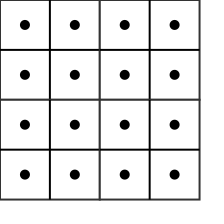
\includegraphics[width=0.5\linewidth, center]{uniform_sampling}
  \caption{Uniform Super-Sampling}
  \label{fig:subim1}
\end{subfigure}
\begin{subfigure}{0.5\textwidth}
  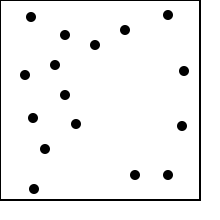
\includegraphics[width=0.5\linewidth, center]{jittered_sampling}
  \caption{Jittered Super-Sampling}
  \label{fig:subim2}
\end{subfigure}
\caption{Diagrams illustrating how samples are distributed within a pixel for
the uniform and jittered sampling methods}
\label{fig:image2}
\end{figure}


%*******************************************************
% Texture Mapping
%*******************************************************
\section{Texture Mapping}

A texture mapping is enabled by setting a texture image to a
\verb|GeometryNode|. This can be with the following Lua command:
\begin{lstlisting}
  set_texture(<filename>)
\end{lstlisting}
This command sets the texture image on the \verb|PhongMaterial| attached to the
\verb|GeometryNode|. 

Texture mapping is implemented by generating $uv$ texture coordinates for each
of the primitives on an intersection. The texture coordinates are then used to
index into the texture map to produce a diffuse colour to be applied to the
intersection point in the lighting calculations. The following subsections
describe the $uv$ generation methods for each of the primitives and the texture
map sampling algorithm.

\subsection{Generating $uv$ Texture Coordinates}

The $uv$ texture coordinates are 2D coordinates with each coordinate having a
value in the range $[0, 1]$. This section will describe how these coordinates
are generated for each of the primitives.

\subsubsection*{Cone}
The texture coordinates for the cone primitive are calculated as follows:
\begin{equation}
\end{split}
  u &= \frac{acos(Q \cdot \begin{bmatrix} 1.0 & 0.0 & 0.0 \end{bmatrix}^{T})}
  {\pi} \\
  v &= \frac{Q_{z}}{h}
\end{split}
\end{equation}
Where $Q$ is the intersection point on the cone and $h$ is the height of the
cone. Essentially, the $u$ coordinate is the angle of rotation of the vector 
(from the origin to the intersection point) about the $z$-axis divided by $\pi$ 
in order to scale it to the range $[0, 1]$. The $v$ coordinate is calculated by
dividing the $z$ coordinate of the intersection point by the height (since the
cone is aligned along the $z$-axis).

\subsubsection*{Cylinder}
The texture coordinates for the cylinder primitive are generated in a similar
fashion as the cone:
\begin{equation}
\begin{split}
  u &= \frac{acos(\begin{bmatrix} Q_{x} & Q_{y} & 0.0 \end{bmatrix|^{T} \cdot 
  \begin{bmatrix} 1.0 & 0.0 & 0.0 \end{bmatrix}^{T})}{\pi} \\
  v &= \frac{Q_{z}}{h} + 0.5
\end{split}
\end{equation}
Note that the finite cyclinder is defined over $\frac{-h}{2} < z < \frac{h}{2}$,
thus it is necessary to add the $0.5$ term to the $v$ coordinate in order to
produce a value in the range of $[0, 1]$.

\subsubsection*{Disc}
Since the disc lies on the $xy$-plane, the texture coordinates are generated
with the following equation:
\begin{equation}
\begin{split}
  u &= \frac{Q_{x}}{2r} + 0.5 \\
  v &= \frac{Q_{y}}{2r} + 0.5 \\
\end{split}
\end{equation}
Where $r$ is the radius of the disc. The $0.5$ term is added to each coordinate 
since the diameter of the disc ranges from $[-r, r]$.

\subsubsection*{Plane}
Since the bounded plane lies on the $xz$-plane, the texture coordinates are
generated as follows:
\begin{equation}
\begin{split}
  u &= \frac{Q_{x}}{s} + 0.5 \\
  v &= \frac{Q_{z}}{s} + 0.5 
\end{split}
\end{equation}
Where $s$ is the dimension of the plane (width and height are equal). 

\subsubsection*{Torus}
To find the $uv$ coordinates for the torus we first need to define two angles.
\begin{equation}
\begin{split}
  \theta &= asin(\frac{Q_{z}}{r}) \\
  \phi &= asin(\frac{Q_{y}}{R + rcos(\theta)})
\end{split}
\end{equation}
Where $r_{0}$ is the major radius and $r_{1}$ is the minor radius. The geometric
representation of the angles are given in Figure~\ref{fig:image3}. Essentially,
$\theta$ is the angle around the tube of the vector from the center of the 
torus' tube to the intersection point. The angle $\phi$ is the radial angle of
the vector from the origin to the intersection point.

\begin{figure}[ht]
  \includegraphics[width=0.5*\textwidth, center]{torus}
  \caption{Illustration of the geometric meaning of the angles \theta and \phi}
  \label{fig:image3}
\end{figure}

Using the two angles we can then generate the $uv$ coordinates as follows:
\begin{equation}
\begin{split}
  u &= \frac{\phi}{\pi} + 0.5 \\
  v &= \frac{\theta}{\pi} + 0.5
\end{split}
\end{equation}

\subsection{Sampling the Texture Map}
Once the $uv$ coordinates are generated, they are used to index into the texture
map to retrieve a colour value:
\begin{equation}
\begin{split}
  i &= \floor*{u(w - 1)} \\
  j &= \floor*{v(h - 1)}
\end{split}
\end{equation}
Where $w$ and $h$ are the width and height of texture map, respectively.

However, this does not produce very nice images since the $uv$ coordinates may
in fact index in between pixels in the texture map. A simple method to solve
this issue is to use bilinear filtering (Blinn \& Newell, 1976). The idea is to
take a weighted average of the surrounding four pixels of the texture coordinate
(Figure~\ref{fig:image4}). The closer the texture coordinate is to a pixel in
the texture map, the larger the weight of that pixel on the final colour.

\begin{figure}[ht]
  \includegraphics[width=0.5*\textwidth, center]{bilinear_filtering}
  \caption{$C_{00}$, $C_{01}$, $C_{10}$, $C_{11}$ represent the colour of the
  surrounding pixels. The area of the four rectangles created by the $uv$ 
  texture coordinate are used as the weights for the colour values.}
  \label{fig:image4}
\end{figure}

Thus, the colour, $C$, can be calculated using bilinear filtering as follows:
\begin{equation}
\begin{split}
  u_{p} = u(w - 1) - i \\
  v_{p} = v(h - 1) - j \\
  C = (1 - u_{p})(1 - v{p})C_{00} + (1 - u_{p})(v_{p})C_{01} + (u_{p})(1 -
  v_{p})C_{10} + (u_{p})(v_{p})C_{11}
\end{split}
\end{equation}


%*******************************************************
% Bump Mapping
%*******************************************************
\section{Bump Mapping}
%*******************************************************
% Refraction
%*******************************************************
\section{Refraction}

Refraction is supported with the optional \verb|<ni>| parameter in the
\newline \verb|gr.material| command. The parameter specifies the index 
of refraction of the material and is used in the refraction calculations.

Refraction is implemented similarly to mirror reflections. When a ray intersects
and object, a secondary refraction ray is generated and traced recursively.

I assume that the ray always goes from air to material or material to air. Thus,
it is necessary to first determine if the ray is entering an object or leaving
and object. This can be determined by taking the dot product of the ray's
direction vector, $\vec{D}$,  and the surface normal, $\vec{N}$. If the result 
is positive then the ray is leaving the object. Otherwise, the ray is entering 
the object. We can now define $n_{r} = \frac{n_{i}}{n_{t}}$ where $n_{i}$ is the 
index of refraction of the material that the ray is leaving and $n_{t}$ is the 
index of refraction of the material that the ray is entering. One of these 
indices of refraction will equal to $1.0$ (the index of refraction of air).

To calculate the refraction ray, $\vec{t}$, we must solve the following 
equation (de Greve, 2006):
\begin{equation}
\begin{split}
  \vec{t} = (-n_{r}(\vec{D}\cdot\vec\vec{N}) - \sqrt{1 - n_{r}^2(1 -
  (\vec{D}\cdot\vec{N})^2)})\vec{N} + n_{r}\vec{D}
\end{split}
\end{equation}
However, if the term inside the square root is negative then the refracted ray
undergoes total internal reflection and so the refraction ray will not be
traced.

The \verb|a4_refract| function in \verb|a4.cpp| performs the above calculation
as well calculating the Fresnel coefficient, $R$, using the following formulas:
\begin{equation}
\begin{split}
  a = \vec{D}\cdot\vec{N} \\
  b = 1 - n_{r}^2(1 - a^2) \\
  R_{0} = \frac{an_{i} - bn_{t}}{an_{i} + bn_{t}} \\
  R_{1} = \frac{an_{t} - bn_{i}}{an_{t} + bn_{i}} \\
  R = \frac{R_{0}^2 + R_{1}^2}{2}
\end{split}
\end{equation}
The Fresnel coefficient, $R$, is multiplied by the colour sampled by the
reflection ray and $(1 - R)$ is multiplied by the colour sampled by the
refraction ray to produce the final balanced colour of the secondary rays.


%*******************************************************
% Phong Shading
%*******************************************************
\section{Phong Shading}

Phong shading of meshes is supported with the new Lua command:
\begin{lstlisting}
  gr.tri_mesh(<name>, <verts>, <faces>)
\end{lstlisting}
This command differs from the \verb|gr.mesh| command in that it subdivides the
faces into triangles and generates per-vertex normals on instantiation.

The following subsections describe the triangulation and normal generation
algorithms as well as the ray-triangle intersection and normal interpolation
algorithms. 

\subsection{Face Triangulation}
Triangulating the faces is a simple matter of looping through the faces and then
splitting the face into a triangle fan. The pseudocode of the algorithm is shown
below. A face is defined as holding an array of integers which are indices into
the vertex array.

\begin{lstlisting}[caption={Mesh face triangulation}]
  function triangulate(face_list):
    new_face_list = {}
    for each face in face_list:
      v0 = face[0];
      for i = 2 to face.size():
        new_face_list.append(face(v0, face[i-1], face[i]))
      end
    end
  end
\end{lstlisting}

\subsection{Per-Vertex Normal Generation}
Generating normals per-vertex is done by calculating the normals of each face
and then adding the normal to each of the vertices connecting the face. The
normals are then normalized to produce an averaged normal for each vertex. The
algorithm is shown in the below.

\begin{lstlisting}[caption={Generating per-vertex normals}]
  function generate_normals(face_list, vert_list):
    normal_list = {}
    for each face in face_list:
      normal = (face[1] - face[0]).cross(face[2] - face[0])
      for each index in face_list:
        normal_list[index] = normal_list[index] + normal
      end
    end

    for each normal in normal_list:
      normal.normalized()
    end
  end
\end{lstlisting}

\subsection{Ray-Triangle Intersection \& Normal Interpolation}
A triangle can be defined parametrically by:
\begin{equation}
\begin{split}
  f(u, v) &= wV_{0} + uV_{1} + vV_{2} \\
  w &= 1 - u - v
\end{split}
\end{equation}
The equation can be solved for $u$, $v$, and $w$ using the algorithm described
in \cite{8_möller_trumbore_1997}.

Using the parametric values of $u$, $v$, and $w$ a normal can be determined by
taking the weighted average of the surrounding vertex normals:
\begin{equation}
  \vec{N} = wN_{0} + uN_{1} + vN_{2}
\end{equation}


%*******************************************************
% Perlin Noise
%*******************************************************
\section{Perlin Noise}

Perlin noise can be enabled with the following Lua command:
\begin{lstlisting}
  set_perlin(<type>)
\end{lstlisting}
This sets the perlin texture on the \verb|PhongMaterial| for the specified 
\verb|GeometryNode|.

The Perlin noise algorithm is implemented exactly as described in
\cite{11_perlin_2002}. The noise function follows the reference implementation 
as closely as possibly.

The noise function takes in as input 3D coordinates and produces a floating
point value in the range $[0, 1]$. The algorithm requires that a hash table is
initialized with random variables in order to function properly. The
\verb|Perlin::init()| function is used to initialize this hash table at the
beginning of program execution.

The noise algorithm is performed by using the coordinates of the 3D point to 
retrieve values from the hash table which are in turn used to retrieve the 
gradient vectors of the eight cube corners of the unit integer lattice . The dot 
product of the gradient vectors are then taken with each of the eight unit cube 
corners specified by the given 3D point. These "influence" values are then
trilinearly interpolated using  the three splined interpolation values 
calculated using the fractional components of the 3D coordinates. 

The \verb|Perlin| class also implements three other static functions which
produce natural textures. The \verb|Perlin::marble| function produces marble
like textures. The \verb|Perlin::cloud| function produces cloud like textures
and the \verb|Perlin::wood| function produces wood like textures. These
functions implement algorithms found in \cite{7_kora_2007}. 


%*******************************************************
% Glossy Reflections
%*******************************************************
\section{Glossy Reflections}

Glossy reflections can be enabled by setting the optional 
\newline \verb|<glossy_samples| parameter in the 
\verb|gr.render| Lua command.

Glossy reflections are implemented by perturbing the reflection ray to a random
point inside of a rectangle defined with a normal in the same direction as the
unperturbed reflection ray, $\vec{r}$ and centered at the point $r$ 
\cite{12_shirley_marschner_2009}. Many of these reflection rays are cast per 
pixel as defined by \verb|glossy_samples| parameter.

Thus, the following values must be calculated:
\begin{equation}
\begin{split}
  i = \frac{a}{2} + \zeta_{0}a \\
  j = \frac{a}{2} + \zeta_{1}a
\end{split}
\end{equation}
Where $a$ is the glossiness value and is calculated by $a = \frac{1}{1 + n_{s}}$
and $n_{s}$ is the Phong specular exponent. $\zeta_{0}$ and $\zeta_{1}$ are
uniform random numbers in the range $[0, 1]$.

These values are then used to calculate the perturbed reflection ray:
\begin{equation}
  \vec{r} = r + i\vec{U} + j\vec{V}
\end{equation}
Where $\vec{U}$ and $\vec{V}$ are orthogonal vectors in the plane of the
$a\times a$ rectangle centered at $r$. These vectors can be generated using the
algorithm described in \cite{6_hughes_moller_2005} where the normal vector is
simply in the direction of the unperturbed reflection ray.


%*******************************************************
% Conclusion
%*******************************************************
\pdfbookmark[1]{Conclusion}{conclusion}
\chapter{Conclusion}

% Back Matter
%*******************************************************
% References
%*******************************************************
\pdfbookmark[1]{References}{references}
\addcontentsline{toc}{chapter}{References}
\chapter*{References}

\begin{thebibliography}{13}
  \bibitem{(Blinn, 1978)}
  Blinn, J. (1978). Simulation of wrinkled surfaces. \textit{ACM SIGGRAPH 
  Computer Graphics}, 12(3), 286-292. doi:10.1145/965139.507101


\end{thebibliography}


    
\end{document}